% !TEX program = xelatex
% NC-format manuscript (English only)
% Compile: xelatex manuscript_en.tex
\documentclass[11pt,a4paper]{article}

\usepackage[margin=2.4cm]{geometry}
\usepackage{amsmath,amssymb}
\usepackage{graphicx}
\usepackage{setspace}
\usepackage{parskip}
\usepackage{titlesec}
\usepackage{booktabs}
\usepackage{tabularx}
\usepackage{multirow}
\usepackage{hyperref}
\usepackage{xcolor}
\usepackage{caption}

\setmainfont{Times New Roman}

\titleformat{\section}{\normalfont\large\bfseries}{\thesection}{0.6em}{}
\titleformat{\subsection}{\normalfont\normalsize\bfseries}{\thesubsection}{0.5em}{}

\setlength{\parskip}{0.6em}
\setlength{\parindent}{0pt}
\onehalfspacing

% Figure path
\graphicspath{{../../0414_v4/figures/}}

% Convenience macros
\newcommand{\keff}{\ensuremath{k_{\mathrm{eff}}}}
\newcommand{\Eint}{\ensuremath{E_{\mathrm{intercept}}}}
\newcommand{\Eslope}{\ensuremath{E_{\mathrm{slope}}}}
\newcommand{\abase}{\ensuremath{\alpha_{\mathrm{base}}}}
\newcommand{\aslope}{\ensuremath{\alpha_{\mathrm{slope}}}}
\newcommand{\kref}{\ensuremath{k_{\mathrm{ref}}}}
\newcommand{\Tref}{\ensuremath{T_{\mathrm{ref}}}}
\newcommand{\kslope}{\ensuremath{k_{\mathrm{slope}}}}

\title{\textbf{Bayesian Neural Surrogates Unify Uncertainty Propagation,\\
Sensitivity Attribution and Calibration for Coupled\\
Multi-Physics Reactor Analysis}}
\author{Yinuo Chen\textsuperscript{1,2},
Sicheng Wang\textsuperscript{2,3},
Xiaojing Liu\textsuperscript{1,2*},
Tengfei Zhang\textsuperscript{1,2*}\\[0.5em]
\small 1.~School of Nuclear Science and Engineering, Shanghai Jiao Tong University,
Shanghai 200240, China\\
\small 2.~Shanghai Digital Nuclear Reactor Technology Integration Innovation Center,
Shanghai 200240, China\\
\small 3.~College of Smart Energy, Shanghai Jiao Tong University,
Shanghai 200240, China\\[0.3em]
\small *~Corresponding authors: \texttt{zhangtengfei@sjtu.edu.cn}; \texttt{xiaojingliu@sjtu.edu.cn}}
\date{NC Draft \textperiodcentered{} \today}

\begin{document}
\maketitle

% ======================================================================
\section*{Abstract}
% ======================================================================

We train a Bayesian neural network (BNN) surrogate on coupled
OpenMC--FEniCS data of a heat-pipe-cooled microreactor and use its
posterior predictive distribution as the single probabilistic object on
which forward uncertainty propagation, Sobol sensitivity attribution and
MCMC posterior calibration all operate, without retraining or
recalibration between analyses. Two-way neutronic--thermal--structural
coupling damps stress variability by approximately 28\% relative to a
decoupled prediction; stress and reactivity are governed by largely
separate material parameters (\Eint{} and \abase{}, respectively); and
across 18 benchmark calibrations the posterior contracts toward
observation-compatible regions with 90\%-CI coverage of 0.917. Each
posterior predictive draw costs approximately $1.76\times 10^{5}$ times
less than a coupled high-fidelity solve, enabling the full uncertainty
workflow to run end-to-end on a single workstation. The
posterior-predictive framework is directly applicable to other coupled
multi-physics systems.

% ======================================================================
\section{Introduction}
% ======================================================================

Microreactors---compact, transportable fission systems rated at
1--20\,MW$_\mathrm{e}$---are being developed for decentralized power
generation in remote communities, defense installations and space
missions\textsuperscript{1,11}. NASA and DOE are advancing fission
surface-power systems for sustained lunar and planetary
operations\textsuperscript{12}, while rapidly growing electricity demand
from AI-intensive data centres reinforces the case for distributed,
dispatchable zero-carbon generation\textsuperscript{13}. Unlike
conventional large-scale plants, these designs concentrate fission power,
heat removal and structural loading within a compact monolithic core
where neutronics, heat transfer and structural mechanics are tightly
coupled through two-way feedback\textsuperscript{1,2}. A single
uncertain material parameter can simultaneously alter the neutronic
balance, the thermal field and the stress state; the closed feedback
loop may amplify or damp the resulting variability in ways that
single-physics analyses cannot capture. The uncertainty problem in these
systems is therefore inherently coupled.

High-fidelity coupled solvers now exist for these systems: MOOSE-based
toolchains handle neutronics--thermo-mechanics--heat-pipe coupling for
KRUSTY-class and larger designs\textsuperscript{2,3}, and
thermal--structural analyses have established stress concentration as a
persistent safety concern in monolithic-core
configurations\textsuperscript{4,5}. Surrogate-assisted probabilistic
modules in the MOOSE ecosystem\textsuperscript{6,7} and digital-twin
pipelines\textsuperscript{8} address forward propagation, sensitivity or
calibration individually, but each uses a separately constructed model
with no shared probabilistic basis between analyses.

Running the full probabilistic workflow---forward uncertainty
propagation, global sensitivity analysis and Bayesian
calibration---directly on the coupled solver is impractical at
${\sim}10^{3}$\,s per solve. Gaussian-process and polynomial-chaos
surrogates face dimensionality constraints in nonlinear coupled settings;
physics-informed neural networks require a closed residual form that
iterative solver exchange does not supply; deterministic neural networks
produce only point predictions. None of these provides the coherent
predictive distribution that all three analyses require.

A Bayesian neural network (BNN) fills this gap. By placing a
distribution over the network weights, a BNN yields a posterior
predictive distribution that can be sampled at negligible cost once
trained. This single distribution serves as the shared probabilistic
layer on which forward propagation, variance-based sensitivity
attribution and observation-conditioned posterior calibration all
operate, with no retraining or recalibration between them.

This paper presents a BNN-based posterior-predictive framework for
end-to-end probabilistic analysis of coupled multi-physics systems. The
framework unifies forward uncertainty propagation, Sobol sensitivity
decomposition and MCMC posterior calibration on a single predictive
layer trained on coupled OpenMC--FEniCS data of a heat-pipe-cooled
reactor. It reveals that two-way coupling damps stress variability by
approximately 28\%, that stress and reactivity are governed by largely
separate parameter pathways, and that the posterior calibration contracts
the material-parameter distribution toward observation-compatible
regions---all at five orders of magnitude less cost per evaluation
than a coupled high-fidelity solve.

% ======================================================================
\section{Results}
% ======================================================================

\subsection{Surrogate accuracy and calibration}

The framework rests on a single BNN that predicts all 15 coupled and
decoupled outputs simultaneously; if this surrogate is inaccurate, the
downstream propagation, sensitivity and calibration results are
unreliable. We evaluated the physics-regularized BNN alongside a
reference (unconstrained) BNN and two conventional baselines---MC-Dropout
and a five-member deep ensemble---on 435 held-out test samples (Table~1,
Fig.~1). Results for the physics-regularized BNN are reported as
mean $\pm$ s.d.\ across 5 random seeds; ablation across four BNN
variants is in Supplementary Table~S3.

On coupled peak global stress the physics-regularized BNN achieves
$R^2 = 0.935 \pm 0.007$ (RMSE $7.63 \pm 0.47$\,MPa), comparable to
MC-Dropout ($R^2 = 0.934$) and deep ensemble ($R^2 = 0.934$). The BNN
advantage is most pronounced on temperature outputs: for maximum fuel
temperature the BNN RMSE is $4.26 \pm 0.18$\,K versus 4.50\,K for both
baselines, and the expected calibration error (ECE) is 0.027 versus
0.183 (MC-Dropout) and 0.190 (deep ensemble)---a five- to six-fold
improvement in calibration quality (Fig.~1A,~C).

The 90\% predictive intervals are conservatively calibrated across all
outputs (PICP 0.937--1.000), and incorporating physics-prior monotonicity
constraints tightens the intervals relative to the unconstrained
reference without reducing coverage (Supplementary Table~S3). The
continuous ranked probability score (CRPS) is lowest for the
physics-regularized BNN on four of five primary outputs (Table~1).

\begin{figure}[htbp]
\centering
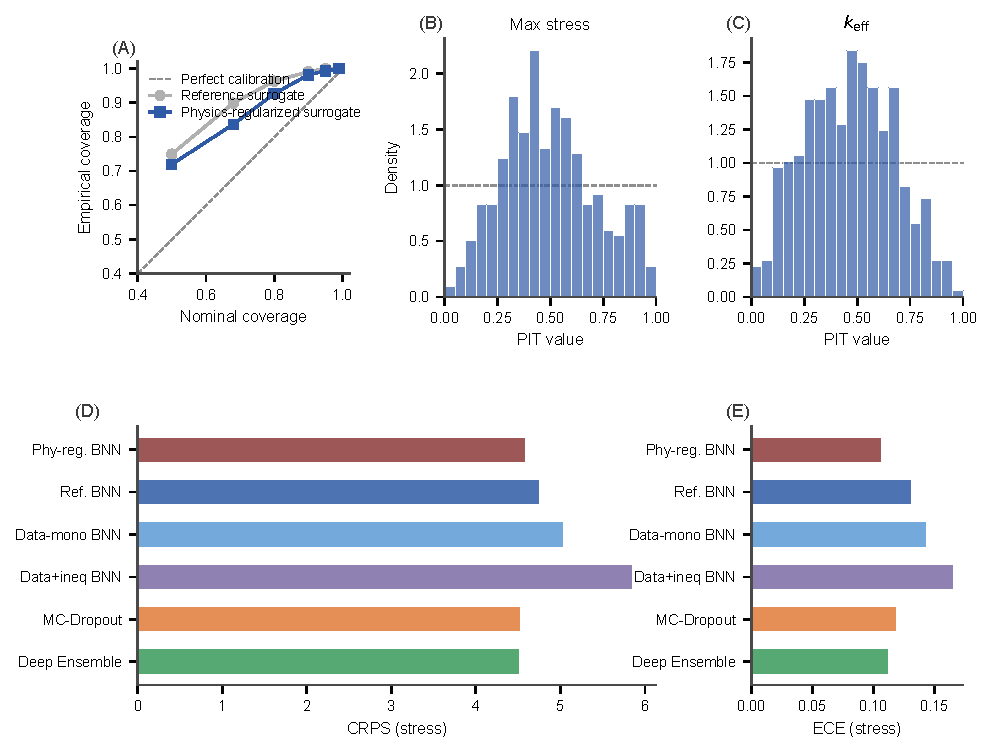
\includegraphics[width=\textwidth]{fig1_accuracy.pdf}
\caption{\textbf{Surrogate accuracy and uncertainty calibration.}
(\textbf{A})~Predicted vs.\ true values for five primary coupled outputs
(physics-regularized BNN, 435 test samples).
(\textbf{B})~Residual distributions.
(\textbf{C})~Calibration curves comparing BNN, MC-Dropout and deep
ensemble. The BNN achieves five- to six-fold lower ECE than the baselines
on temperature outputs.}
\label{fig:accuracy}
\end{figure}

% --- Table 1: Full accuracy comparison ---
\begin{table}[htbp]
\centering
\caption{\textbf{Surrogate accuracy on five primary coupled outputs.}
Physics-regularized BNN: mean $\pm$ s.d.\ across 5 seeds; external
baselines: single run. Bold CRPS indicates best per output.}
\label{tab:accuracy}
\smallskip
\small
\begin{tabular}{lccccc}
\toprule
Output & $R^2$ & RMSE & PICP & ECE & CRPS \\
\midrule
\multicolumn{6}{l}{\textit{Physics-regularized BNN}} \\
\quad \keff{}
  & $0.633 \pm 0.258$
  & $0.0006 \pm 0.0004$
  & $0.981 \pm 0.007$
  & 0.123
  & \textbf{0.0002} \\
\quad Max.\ fuel temp.
  & $0.621 \pm 0.044$
  & $4.26 \pm 0.18$\,K
  & $0.936 \pm 0.015$
  & 0.027
  & \textbf{2.39} \\
\quad Max.\ monolith temp.
  & $0.622 \pm 0.044$
  & $4.80 \pm 0.20$\,K
  & $0.942 \pm 0.013$
  & 0.031
  & \textbf{2.70} \\
\quad Max.\ global stress
  & $0.935 \pm 0.007$
  & $7.63 \pm 0.47$\,MPa
  & $0.987 \pm 0.007$
  & 0.106
  & \textbf{4.58} \\
\quad Wall expansion
  & $0.993 \pm 0.001$
  & $0.0020 \pm 0.0002$
  & $1.000 \pm 0.000$
  & 0.194
  & 0.0017 \\
\midrule
\multicolumn{6}{l}{\textit{MC-Dropout}} \\
\quad Max.\ fuel temp.
  & 0.590  & 4.50\,K  & ---  & 0.183  & 2.62 \\
\quad Max.\ global stress
  & 0.934  & 7.66\,MPa  & ---  & 0.118  & 4.52 \\
\midrule
\multicolumn{6}{l}{\textit{Deep Ensemble (5 members)}} \\
\quad Max.\ fuel temp.
  & 0.590  & 4.49\,K  & ---  & 0.190  & 2.63 \\
\quad Max.\ global stress
  & 0.934  & 7.64\,MPa  & ---  & 0.112  & 4.50 \\
\bottomrule
\end{tabular}
\end{table}


\subsection{Physics consistency}

We verified the BNN's adherence to known physical relationships through
two tests: monotonicity verification against 15 input--output pairs
derived from the constitutive laws, and inequality constraint
satisfaction (Fig.~2A). For all high-confidence monotonicity
pairs---including the dominant stress drivers \Eint{} (+), \abase{} (+),
and \kref{} ($-$)---all four BNN variants achieved zero violation rates
on the 435 held-out test samples using discrete $\pm\delta$ perturbation
testing. The only non-trivial violations occurred for the
medium-confidence pair SS316\_$\alpha$ $\to$ fuel temperature (36--54\%
across models), reflecting a weaker and potentially nonlinear
relationship that the training data does not consistently support. All
four models also satisfied ordering constraints
(max $\geq$ average temperature) and non-negativity constraints
(stress $\geq 0$) with zero violations.

Decomposing total predictive variance into epistemic
(weight-uncertainty) and aleatoric (observation-noise) components
revealed that aleatoric uncertainty dominates across all outputs,
accounting for 58--90\% of total variance (Fig.~2B). The epistemic
fraction was highest for wall expansion (${\sim}42\%$) and stress
(${\sim}30\%$), indicating greater model-form uncertainty for these
mechanically driven outputs.

\begin{figure}[htbp]
\centering
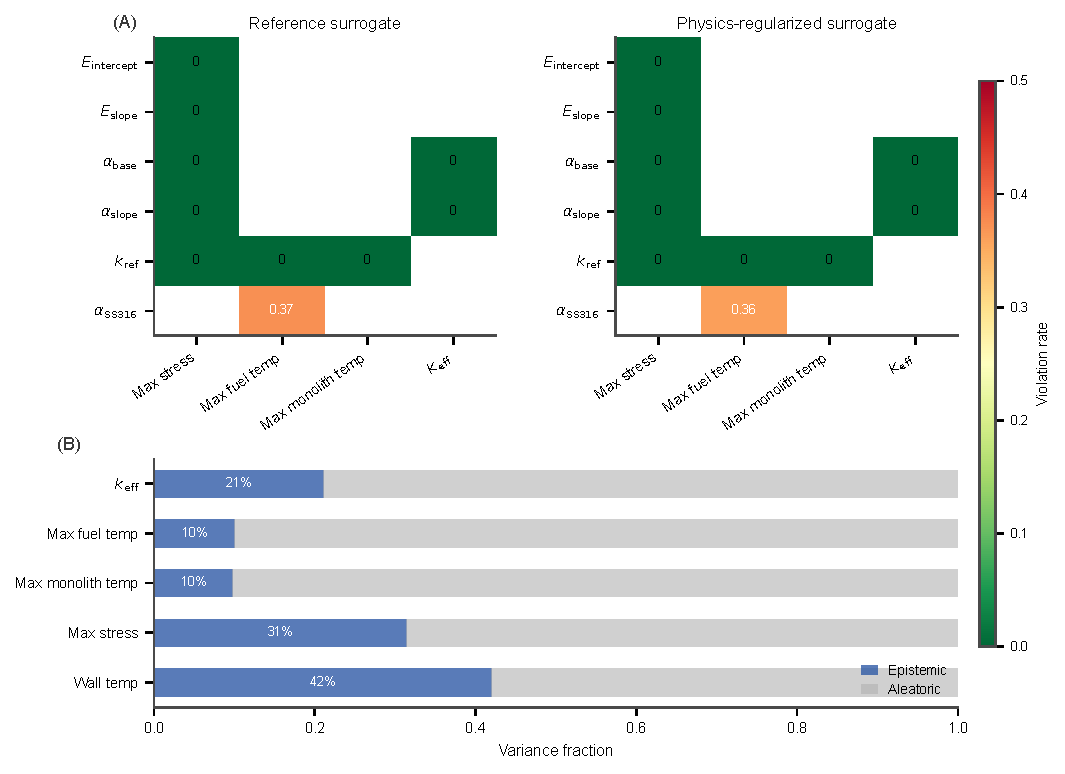
\includegraphics[width=\textwidth]{fig5_physics.pdf}
\caption{\textbf{Physics consistency verification.}
(\textbf{A})~Monotonicity violation rates for 15 input--output pairs
across four BNN variants; high-confidence pairs achieve zero violations.
(\textbf{B})~Epistemic vs.\ aleatoric variance decomposition across
five primary outputs.}
\label{fig:physics}
\end{figure}


\subsection{Forward uncertainty propagation}

Propagating 20,000 Latin hypercube samples through the BNN posterior
predictive mean yields a coupled stress distribution with mean
162.5\,MPa and standard deviation 35.5\,MPa, versus a decoupled mean of
202.4\,MPa and standard deviation of 49.2\,MPa. Coupling reduces the
stress standard deviation by approximately 28\% and lowers the mean by
approximately 40\,MPa (Table~2, Fig.~3).

The coupled \keff{} has mean 1.1036 and standard deviation approximately
107\,pcm. The decoupled \keff{} is effectively constant because, at the
reference geometry, the sampled material parameters do not enter the
neutronic cross-section tables; all coupled \keff{} variability
originates from thermal-expansion modification of core geometry.

\begin{table}[htbp]
\centering
\caption{\textbf{Forward UQ summary: coupled vs.\ decoupled distributions}
(20,000 LHS samples through BNN posterior predictive mean).}
\label{tab:forward}
\smallskip
\begin{tabular}{lcccc}
\toprule
Output & Coupled mean & Coupled s.d. & Decoupled mean & Decoupled s.d. \\
\midrule
Stress (MPa) & 162.5 & 35.5 & 202.4 & 49.2 \\
\keff{} & 1.1036 & 0.00107 & $\sim$constant & $\sim$0 \\
\bottomrule
\end{tabular}
\end{table}

\begin{figure}[htbp]
\centering
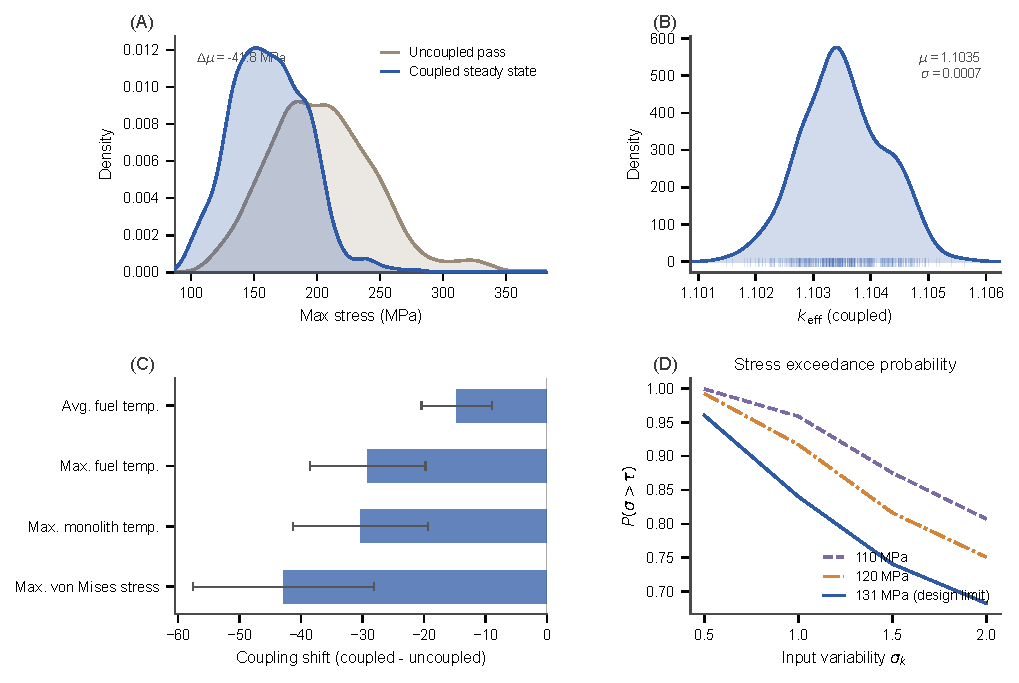
\includegraphics[width=\textwidth]{fig3_forward.pdf}
\caption{\textbf{Forward uncertainty propagation.}
Coupled vs.\ decoupled output distributions for stress and \keff{}.
Two-way coupling reduces the stress standard deviation by ${\approx}28\%$
and introduces \keff{} variability that is absent in the decoupled case.}
\label{fig:forward}
\end{figure}


\subsection{Global sensitivity analysis}

Sobol analysis (50 independent replications, $N_S = 4096$ per matrix;
full index table in Supplementary Table~S4) shows that stress and
\keff{} are governed by two largely separate physical pathways
(Table~3, Fig.~4).

Stress is rooted in the elastic-constitutive pathway. \Eint{} alone
accounts for approximately 55\% of the first-order variance
($S_1 = 0.548$, 90\% CI [0.498, 0.572]), and the near-zero gap between
its total-order and first-order indices indicates that it acts with
minimal interaction. Secondary contributors---\abase{}
($S_1 = 0.210$), \kref{} and $\nu$---add a collective approximately
15\%, while the remaining parameters are negligible. The dominance of
\Eint{} is a direct consequence of the generalised Hooke's law:
stiffness enters the stress field linearly.

\keff{} is rooted in the thermal-expansion pathway. \abase{} accounts
for approximately 77\% of the first-order variance
($S_1 = 0.771$, 90\% CI [0.747, 0.788]): it sets the magnitude of
geometric expansion, which alters neutron leakage and shifts the
neutronic balance. \aslope{} contributes a further approximately 19\%
($S_1 = 0.195$), while no elasticity or conductivity parameter has a
first-order effect on reactivity above the noise floor.

The two pathways share almost no dominant parameters. This separation
means that stress and \keff{} observations constrain different regions
of the material-parameter space---an important constraint for any
monitoring strategy that aims to reduce material-property uncertainty.

\begin{table}[htbp]
\centering
\caption{\textbf{First-order Sobol indices $S_1$ for stress and \keff{}}
(physics-regularized BNN, $N_S = 4096$, 50 replications, 90\% CI).
Only factors with CI lower bound $> 0$ are shown.}
\label{tab:sobol}
\smallskip
\begin{tabular}{lcc}
\toprule
Parameter & Stress $S_1$ [90\% CI] & \keff{} $S_1$ [90\% CI] \\
\midrule
\Eint{}   & 0.548 [0.498, 0.572] & --- \\
\abase{}  & 0.210 [0.171, 0.254] & 0.771 [0.747, 0.788] \\
$\nu$     & 0.063 [0.034, 0.097] & --- \\
\kref{}   & 0.065 [0.014, 0.118] & --- \\
\aslope{} & --- & 0.195 [0.112, 0.250] \\
\bottomrule
\end{tabular}
\end{table}

\begin{figure}[htbp]
\centering
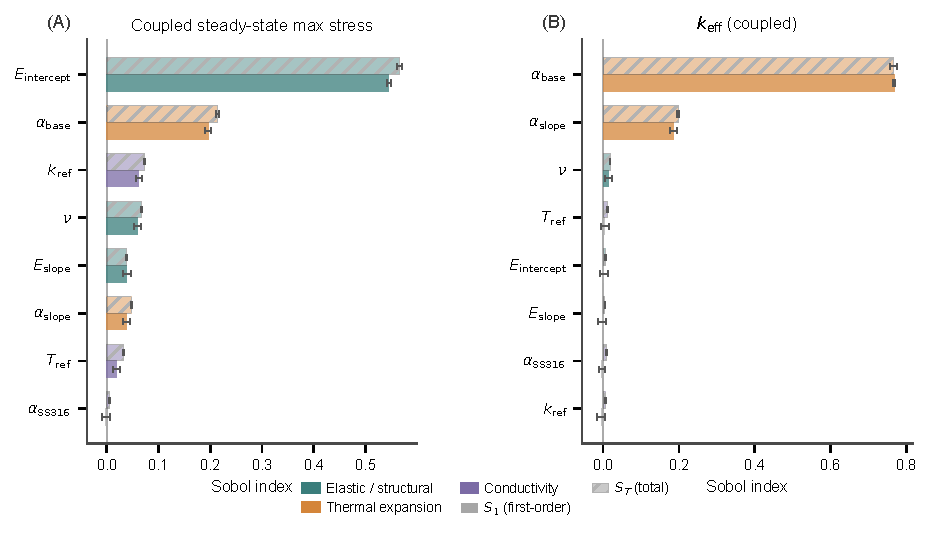
\includegraphics[width=\textwidth]{fig4_sobol.pdf}
\caption{\textbf{Sobol sensitivity analysis.}
First-order and total-order indices for stress and \keff{} reveal two
largely separate physical pathways: the elastic-constitutive pathway
(dominated by \Eint{}) for stress, and the thermal-expansion pathway
(dominated by \abase{}) for \keff{}.}
\label{fig:sobol}
\end{figure}


\subsection{Posterior calibration}

Bayesian calibration uses the same BNN to update the prior parameter
distribution given noisy observations. The four calibrated
parameters---\Eint{}, \abase{}, \aslope{} and \kref{}---are the four
that the Sobol analysis identified as covering the dominant variance
channels for stress and \keff{}. Metropolis--Hastings MCMC is run on 18
benchmark cases drawn from the test split (6 low / 6 near / 6 high
stress; details in Methods) with 4 independent chains per case.

Chain convergence was assessed using rank-normalised split-$\hat{R}$
(Vehtari et al.\ 2021) and Geyer initial-positive-sequence effective
sample size. Across all 72 parameter--case combinations for the
physics-regularized BNN, $\hat{R}_{\max} = 1.017$ (well below the 1.1
threshold), $\mathrm{ESS}_{\min} = 352$, and mean acceptance rate
$= 0.605$ (Fig.~5A--B; Supplementary Figs.~S9--S10 and Supplementary
Table~S5).

Across the 18 cases, the posterior 90\%-CI coverage is 0.917---the
observations successfully constrain the parameters that the Sobol
analysis flagged as most influential. In higher-stress cases, the
\Eint{} marginal shifts toward larger values, consistent with its
dominant role in the elastic-constitutive pathway. The joint posterior of
\Eint{} and \abase{} develops a compensation ridge: an increase in
stiffness can be partially offset by a decrease in thermal expansion,
leaving the stress product $\sigma \sim E \cdot \alpha \cdot \Delta T$
approximately invariant. This partial non-identifiability arises from
the multiplicative structure and would not be visible in a single-output
calibration (Fig.~5).

At the posterior-mean parameters of each case, the BNN-predicted stress
tracks the true value with MAE $= 10.4$\,MPa over a true-stress range
of 102--198\,MPa. Prior sensitivity analysis (6 prior configurations)
and observation noise sensitivity analysis (noise fraction 0.5--10\%)
confirmed the robustness of posterior inference (Supplementary
Figs.~S14--S15, Tables~S11--S12).

\begin{figure}[htbp]
\centering
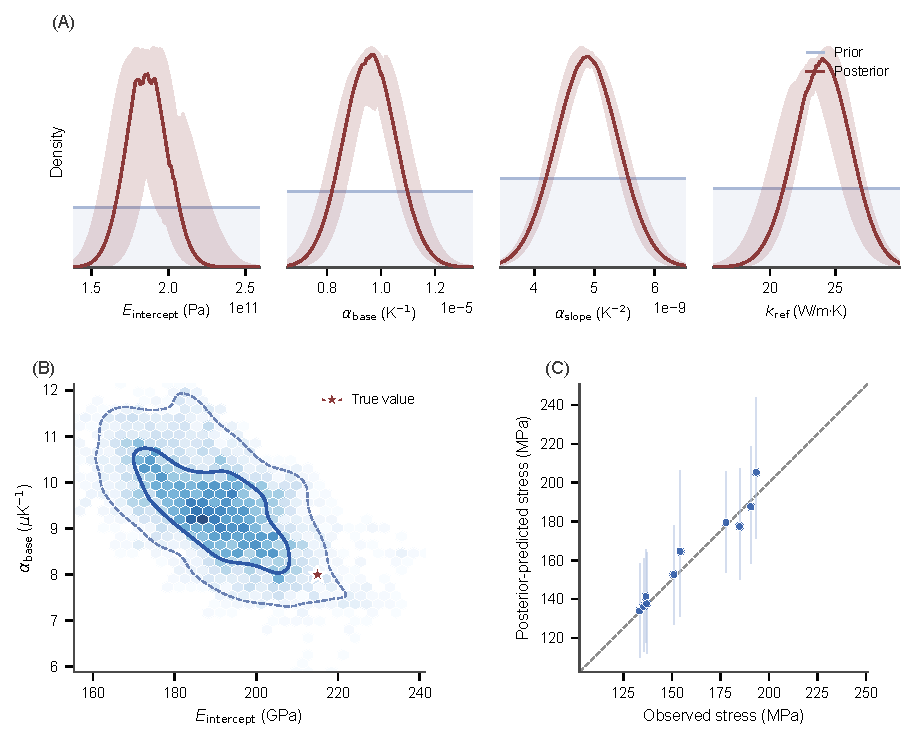
\includegraphics[width=\textwidth]{fig6_posterior.pdf}
\caption{\textbf{Posterior calibration results.}
(\textbf{A})~MCMC convergence diagnostics (split-$\hat{R}$ and ESS).
(\textbf{B})~Acceptance rates across 18 benchmark cases.
(\textbf{C})~Marginal posterior distributions for \Eint{} and \abase{}
in representative low-, near-, and high-stress cases.
(\textbf{D})~Joint posterior of \Eint{} vs.\ \abase{} showing the
compensation ridge.}
\label{fig:posterior}
\end{figure}


\subsection{Computational efficiency}

The BNN produces one posterior-predictive draw (averaged over 50 Monte
Carlo weight samples) in $1.29 \times 10^{-2}$\,s on GPU. Batched
inference at batch size 1024 reaches a per-sample cost of
$1.34 \times 10^{-5}$\,s, equivalent to a throughput of approximately
$7.5 \times 10^{4}$\,samples/s. The coupled HF solver requires
2266\,s (mean of three independent runs, s.d.\ 1.34\,s; AMD EPYC 9654
96-core node, 566\,GB RAM, $2\times$ RTX 5090). The resulting speedup is
approximately $1.76 \times 10^{5}$ for one posterior-predictive draw and
approximately $1.69 \times 10^{8}$ for batched per-sample inference.
A 20,000-sample forward-UQ pass requires approximately 0.3\,s of GPU
time, against $4.5 \times 10^{7}$\,s of sequential HF cost. This speedup
enables the full probabilistic workflow---20,000-sample Monte Carlo
propagation, 50-replication Sobol analysis, and 18-case MCMC
calibration---to run within minutes of wall-clock time.

The BNN also exploits limited training data efficiently. With only 507
training samples (25\% of the full training set), the surrogate achieves
RMSE $= 4.93$---96\% of its peak performance at full data utilisation
(RMSE $= 4.62$). Marginal improvement from 50\% to 100\% data is less
than 1\% (Fig.~6).

% ======================================================================
\section{Discussion}
% ======================================================================

The stress standard deviation drops from approximately 49.2\,MPa in the
decoupled response to approximately 35.5\,MPa after coupling
convergence, a roughly 28\% reduction. The mechanism is the negative
neutronic--thermal feedback characteristic of compact monolithic-core
systems: thermal expansion modifies the core geometry, which shifts the
neutronic balance and partially offsets the direct stress increase. What
the BNN-based forward propagation establishes is the net effect of this
feedback on the output distribution. A decoupled analysis does not see
the feedback loop and therefore overestimates the parameter-driven stress
variability. The overestimate is conservative for safety-margin
evaluation and cannot produce an unsafe conclusion, but it inflates the
apparent penalty of material-property uncertainty. In practice, this can
translate into manufacturing tolerances stricter than the coupled
response warrants.

Compared with an ELBO-only BNN (Supplementary Table~S3), adding
physics-prior monotonicity constraints shrinks the 90\% predictive
interval without reducing coverage. The primary model enforces
monotonicity relations derived from the physics of the constitutive
laws---for example, that stress increases with Young's modulus at
fixed thermal strain. The interval tightening at constant coverage
indicates genuine sharpening rather than miscalibration, and the same
posterior predictive distribution propagates consistently through
forward UQ, Sobol attribution and MCMC calibration. A point-estimate
surrogate would require separate uncertainty wrappers for each analysis
with no guarantee of mutual consistency.

The sensitivity and calibration results have practical consequences for
the engineering workflow. For stress-margin assessment, tightening the
uncertainty on \Eint{}---e.g.\ through coupon tensile tests at
operating temperature---is the single highest-leverage action; for
reactivity stability, dilatometry to refine \abase{} is the priority.
Because these two measurements target different experimental setups,
they can proceed in parallel. When measured data become available, the
posterior calibration folds that information into the same surrogate
without retraining. If a posterior update reveals that a safety margin
is tighter than initially expected, the Sobol ranking identifies which
parameter to prioritise in the next round of characterisation. The
near-zero parameter overlap between the stress and \keff{} pathways
means that a calibration protocol combining both outputs provides
stronger parameter identification than either alone. These indications
are model-driven and require verification on the high-fidelity solver
before adoption as design directives.

The surrogate is trained on data from a single HPR design point; a
different geometry, fuel enrichment or operating envelope would require
regenerating the training set and retraining. The methodology itself is
not design-specific: the same workflow of coupled-data generation, BNN
training and three-stage probabilistic analysis is directly applicable
to other reactor types and other coupled multi-physics systems. The MCMC
calibration fixes four parameters at their true values and calibrates
the remaining four; extending to a full eight-parameter calibration
would require additional independent observations. The \keff{} surrogate
degrades on out-of-distribution \abase{} tails ($R^2$ drops to
approximately 0.29 versus 0.825 in-distribution; Supplementary
Fig.~S5), so the Sobol and posterior conclusions for \keff{} hold only
within the training range. All posterior summaries are computed on the
surrogate side. An independent high-fidelity re-evaluation at the
posterior-mean parameter vectors is documented separately. The present
study uses synthetic observations constructed from the high-fidelity
solver; if experimental or monitoring data become available, the same
calibration workflow can ingest real observations directly.

% ======================================================================
\section{Methods}
% ======================================================================

\subsection{Material uncertainty model}

The coupled HPR simulation involves eight material properties of the
SS316 monolith grouped by physical function: structural mechanics
(\Eint{}, \Eslope{}, $\nu$), thermal deformation (\abase{}, \aslope{}),
and thermal transport (\kref{}, \Tref{}, \kslope{}). All eight are
assigned independent uniform priors with half-width 10\% of the nominal
design value. The same prior distribution is used throughout: as the
sampling distribution in forward UQ, as the input domain for Sobol
analysis, and as the prior in posterior calibration. Full parameter
definitions, nominal values and constitutive-law relationships are in
Supplementary Note~E and Supplementary Table~S1.

\subsection{Coupled high-fidelity simulation}

The high-fidelity workflow couples OpenMC Monte Carlo neutronics with the
FEniCS finite-element solver through a Picard fixed-point iteration
scheme\textsuperscript{9}. Two fidelity levels are retained: a decoupled
single-pass prediction before coupling convergence and a coupled
steady-state prediction after full convergence. Each HF evaluation
produces 15 scalar outputs. A dataset of $n = 2900$ samples was
generated by Latin hypercube sampling; samples were split into training
(2029), validation (436) and test (435) sets with a fixed random seed
(seed $= 2026$). The BNN maps directly from the 8 input parameters to
the 15 outputs without resolving intermediate coupling fields. Details
of the iteration scheme, convergence criteria and output definitions are
in Supplementary Note~E.

\subsection{Bayesian neural network surrogate}

The surrogate is a BNN with mean-field variational inference (MFVI,
Bayes-by-Backprop\textsuperscript{10}). The network uses a fully
connected backbone with two output heads: a mean head and a log-variance
head that models heteroscedastic observation noise. Training minimises
the negative evidence lower bound (ELBO). The posterior predictive
distribution at a new input is approximated by Monte Carlo averaging
over $M$ weight samples from the trained variational posterior: at
inference $M = 50$, for Sobol analysis $M = 30$, and for the MCMC
likelihood $M = 20$. Hyperparameters were optimised via Optuna
(Supplementary Table~S2). Physics-prior monotonicity constraints are
incorporated as an auxiliary loss term during training. Full ELBO
derivation, KL annealing schedule and architecture details are in
Supplementary Note~A.

\subsection{Forward uncertainty propagation}

Forward UQ draws $N = 20{,}000$ Latin hypercube samples from the joint
prior and evaluates the BNN posterior predictive mean at each sample.
Using the predictive mean rather than a full predictive draw isolates
parametric uncertainty from the BNN's own epistemic and aleatoric spread;
the predictive-draw variant is reported in Supplementary Note~D.

\subsection{Sobol sensitivity analysis}

Global sensitivity is assessed through variance-based Sobol indices
estimated with the Saltelli cross-matrix scheme ($N_S = 4096$ per
matrix, 40,960 surrogate evaluations per replication). The analysis is
repeated 50 times; a factor is treated as a stable contributor only if
the lower bound of its 90\% CI exceeds zero. Methodological details
including the Jansen estimator definition are in Supplementary Note~B.

\subsection{Posterior calibration}

Posterior calibration uses Bayesian inference:
$p(\boldsymbol{\theta} \mid \mathbf{y}_{\mathrm{obs}}) \propto
p(\mathbf{y}_{\mathrm{obs}} \mid \boldsymbol{\theta})\,
\pi(\boldsymbol{\theta})$, with the likelihood evaluated through the BNN
posterior predictive mean. Four parameters are calibrated (\Eint{},
\abase{}, \aslope{}, \kref{}), selected on the basis of their Sobol
ranking; the remaining four are fixed at their true values. The 18
benchmark cases are drawn from the test split (6 low, 6 near, 6 high
stress). Observations are the true HF outputs of 5 primary coupled
quantities perturbed by 2\% multiplicative Gaussian noise. The posterior
is sampled by Metropolis--Hastings MCMC with 4 independent chains (8000
iterations, burn-in 2000, thinning 5). Implementation details and
convergence diagnostics are in Supplementary Note~C.

% ======================================================================
\section*{Data availability}
% ======================================================================

The coupled simulation dataset and fixed train/validation/test split
used in this study are available at [repository URL upon acceptance].

\section*{Code availability}

The BNN training, evaluation and analysis code are available at
[repository URL upon acceptance].

% ======================================================================
\section*{References}
% ======================================================================

\begin{enumerate}\small
\item McClure PR, Poston DI, Dixon DD, Cooley JW. Design of megawatt
      power level heat pipe reactors. LANL, LA-UR-15-28840; 2015.
\item Stauff NE, et al. High-fidelity multiphysics modeling of a heat
      pipe microreactor using BlueCrab. \textit{Nucl.\ Sci.\ Eng.} 2024.
\item Miao Y, et al. Multiphysics simulation of KRUSTY warm critical
      experiments using MOOSE tools. \textit{Nucl.\ Sci.\ Eng.} 2025.
\item Aldebie F, et al. Thermal-mechanical safety analysis of heat pipe
      micro reactor. \textit{Nucl.\ Eng.\ Des.} 2024;420:113003.
\item Jeong MJ, et al. Multiphysics analysis of heat pipe cooled
      microreactor core. \textit{Front.\ Energy Res.} 2023;11:1213000.
\item Slaughter AE, et al. MOOSE Stochastic Tools. \textit{SoftwareX}.
      2023;22:101345.
\item Dhulipala SLN, et al. MOOSE ProbML. \textit{J.\ Comput.\ Sci.}
      2026;94:102776.
\item Lim JY, et al. A hybrid surrogate modeling framework for the
      Digital Twin of a FHR. \textit{Nucl.\ Eng.\ Des.} 2025;433:113690.
\item Zhang T, Chen Y, Wang S, Liu X. Design-oriented multiphysics
      analysis and surrogate modelling of a heat-pipe-cooled reactor.
      \textit{Energy}. 2025. (in press)
\item Blundell C, et al. Weight uncertainty in neural networks. ICML
      2015; pp.\ 1613--1622.
\item DOE Office of Nuclear Energy. What is a microreactor? 2021.
\item NASA. Fission Surface Power. 2024.
\item IEA. Electricity 2025: Analysis and forecast to 2027. Jan 2025.
\end{enumerate}

% ======================================================================
\section*{Acknowledgements}
% ======================================================================

The authors gratefully acknowledge the support provided by the National
Natural Science Foundation of China [12175138]; Shanghai Rising-Star
Program; and LingChuang Research Project of China National Nuclear
Corporation.

% ======================================================================
\section*{Author contributions}
% ======================================================================

Y.C.\ developed the BNN surrogate model, designed and performed the
experiments, analysed the results and drafted the manuscript. S.W.\
contributed to the coupled simulation framework. X.L.\ and T.Z.\
conceived and supervised the project, provided scientific guidance and
revised the manuscript. All authors discussed the results and approved
the final version.

% ======================================================================
\section*{Competing interests}
% ======================================================================

The authors declare no competing interests.

\end{document}
